%% Supplementary material for the Chaos manuscript (separate PDF, as required by AIP Publishing).
%% Compile after main.tex (cross-references to the article are read from main.aux):
%%   pdflatex supplement && pdflatex supplement
%% Tables in supplement/ and Fig. S1 are generated by experiments/make_supplement.py.
\documentclass[10pt,letterpaper]{article}
\usepackage[utf8]{inputenc}
\usepackage[T1]{fontenc}
\usepackage{mathptmx}
\usepackage{amsmath,amssymb}
\usepackage{graphicx}
\usepackage{booktabs}
\usepackage{array}
\usepackage[margin=2cm]{geometry}
\usepackage[labelsep=period,font=small,justification=justified]{caption}
\usepackage{url}
\usepackage{xr}
\externaldocument[M-]{main}

\renewcommand{\thesection}{S\arabic{section}}
\renewcommand{\thetable}{S\arabic{table}}
\renewcommand{\thefigure}{S\arabic{figure}}
\renewcommand{\theequation}{S\arabic{equation}}
\renewcommand{\figurename}{FIG.}
\renewcommand{\tablename}{TABLE}
\setlength{\parskip}{0pt}
\renewcommand{\arraystretch}{1.12}
\newcommand{\mref}[1]{\ref{M-#1}}

\newcommand{\SGgain}{10.67}
\newcommand{\dcdd}{0.107}
\newcommand{\thrsc}{0.133}
\newcommand{\fracbelow}{23.9}

\newcommand{\torchver}{2.14.0}
\newcommand{\costcpu}{Intel Xeon processor at 2.1~GHz}
\newcommand{\costrows}{1500}
\newcommand{\costsamples}{64}

\newcommand{\symperiods}{200\,000}


\begin{document}

\begin{center}
{\large\textbf{Supplementary Material}}\\[6pt]
{\large From separatrix to strange attractor: Physics-informed normalizing flows for recovering missing dynamics in a spring-coupled inverted pendulum}\\[8pt]
Fredy Alexander Orjuela L\'opez\\[2pt]
{\small Departamento de F\'isica, Universidad de los Andes, Bogot\'a, Colombia}
\end{center}

\bigskip
\noindent This supplementary material contains the complete results of the reconstruction benchmark for every task, missing fraction, and random mask (Sec.~\ref{sec:bench}); the embedding parameters of Sec.~\mref{sec:tasks} and the diagnostics quoted in Sec.~\mref{sec:results} of the article (Sec.~\ref{sec:diag}); the cost benchmark of the flow and the diffusion model (Sec.~\ref{sec:cost}); the symmetry check of the reference attractor (Sec.~\ref{sec:sym}); the diagnostic figures of the five conservative regimes at full size (Sec.~\ref{sec:cases}); and a guide to the laboratory that relates every result to the script that produces it (Sec.~\ref{sec:guide}). Section, equation, figure, and table numbers without the prefix S refer to the article. The tables of Secs.~\ref{sec:bench}--\ref{sec:sym} and Fig.~\ref{fig:emb} are generated from the JSON files of the code archive by the script \texttt{experiments/make\_supplement.py}.

%% ------------------------------------------------------------------------------------------
\section{Complete results of the reconstruction benchmark}\label{sec:bench}

The benchmark of Sec.~\mref{sec:results} comprises four tasks (Sec.~\mref{sec:tasks}), three missing fractions, two random masks per fraction, and up to seven imputers, with the settings of Table~\mref{tab:hyper}. Tables~\ref{tab:C1}--\ref{tab:C0} list every metric for every setting as the mean over the two masks $\pm$ the half-range, so that the values for the two masks are the mean plus and minus the half-range. The correlation $\rho$ and the normalized root-mean-square error (NRMSE) refer to the posterior median; the continuous ranked probability score (CRPS), Eq.~(\mref{eq:crps}), is normalized by the standard deviation of the target; ``cov.'' is the empirical coverage of the central $90\%$ interval; ``sign'' is the fraction of samples with the correct sign of the first target ($\cos\theta$ in C1, $\sin\theta$ in C2 and C3, and $\dot\theta$ in C0); and $W_1$ is the sliced Wasserstein distance between the imputed and true Poincar\'e sections. Each run is evaluated on 1500 missing entries with 64 samples per entry. The static GPR uses only the current value of the complete channel; the original FPRM uses the delay window of the complete channel; the other imputers receive the full conditioning vector, Eq.~(\mref{eq:context}), which includes the forcing phase in task C1 and in the phase variant of task C3. The rows at $90\%$ missing data coincide, after rounding, with Table~\mref{tab:fprm}. The metrics of each individual run, together with its training time and selected checkpoint, are listed in the file \texttt{results/benchmark\_runs.csv} of the code archive.

\begin{table}[!htbp]
\caption{Task C1: collar height and angular velocity, $(c,\dot\theta)$, reconstructed from the complete spring force $s$ on the chaotic attractor. The correlation, NRMSE, CRPS, and coverage are averaged over the two targets.}
\label{tab:C1}
\centering\footnotesize\setlength{\tabcolsep}{4pt}
\begin{tabular}{lcccccc}
\toprule
Imputer & $\rho$ & NRMSE & CRPS & cov. & sign & $W_1$\\
\midrule
\multicolumn{7}{l}{\textit{30\% missing}}\\
static GPR & 0.1230\,$\pm$\,0.0004 & 0.993\,$\pm$\,0.001 & 0.5677\,$\pm$\,0.0021 & 0.910\,$\pm$\,0.006 & 0.550\,$\pm$\,0.006 & 0.5320\,$\pm$\,0.0235\\
original FPRM (GPR) & 0.8707\,$\pm$\,0.0027 & 0.491\,$\pm$\,0.007 & 0.1870\,$\pm$\,0.0015 & 0.915\,$\pm$\,0.009 & 0.869\,$\pm$\,0.002 & 0.0939\,$\pm$\,0.0089\\
GPR (full context) & 0.9943\,$\pm$\,0.0008 & 0.105\,$\pm$\,0.006 & 0.0255\,$\pm$\,0.0019 & 0.907\,$\pm$\,0.012 & 0.988\,$\pm$\,0.002 & 0.0131\,$\pm$\,0.0009\\
cVAE & 0.9985\,$\pm$\,0.0002 & 0.053\,$\pm$\,0.003 & 0.0126\,$\pm$\,0.0004 & 0.966\,$\pm$\,0.000 & 0.992\,$\pm$\,0.002 & 0.0094\,$\pm$\,0.0005\\
DDPM & 0.9994\,$\pm$\,0.0000 & 0.035\,$\pm$\,0.001 & 0.0148\,$\pm$\,0.0001 & 0.974\,$\pm$\,0.000 & 0.992\,$\pm$\,0.001 & 0.0111\,$\pm$\,0.0007\\
NSF & 0.9995\,$\pm$\,0.0001 & 0.031\,$\pm$\,0.002 & 0.0121\,$\pm$\,0.0003 & 0.896\,$\pm$\,0.002 & 0.993\,$\pm$\,0.001 & 0.0087\,$\pm$\,0.0002\\
NSF + physics & 0.9998\,$\pm$\,0.0000 & 0.022\,$\pm$\,0.001 & 0.0106\,$\pm$\,0.0002 & 0.861\,$\pm$\,0.003 & 0.995\,$\pm$\,0.001 & 0.0084\,$\pm$\,0.0000\\
\midrule
\multicolumn{7}{l}{\textit{60\% missing}}\\
static GPR & 0.0878\,$\pm$\,0.0336 & 1.006\,$\pm$\,0.009 & 0.5711\,$\pm$\,0.0036 & 0.903\,$\pm$\,0.001 & 0.548\,$\pm$\,0.002 & 0.5062\,$\pm$\,0.0023\\
original FPRM (GPR) & 0.8811\,$\pm$\,0.0082 & 0.471\,$\pm$\,0.015 & 0.1817\,$\pm$\,0.0085 & 0.922\,$\pm$\,0.006 & 0.871\,$\pm$\,0.003 & 0.0584\,$\pm$\,0.0131\\
GPR (full context) & 0.9791\,$\pm$\,0.0002 & 0.190\,$\pm$\,0.003 & 0.0541\,$\pm$\,0.0015 & 0.894\,$\pm$\,0.001 & 0.961\,$\pm$\,0.001 & 0.0188\,$\pm$\,0.0042\\
cVAE & 0.9816\,$\pm$\,0.0040 & 0.181\,$\pm$\,0.019 & 0.0409\,$\pm$\,0.0041 & 0.925\,$\pm$\,0.004 & 0.960\,$\pm$\,0.004 & 0.0160\,$\pm$\,0.0004\\
DDPM & 0.9969\,$\pm$\,0.0005 & 0.075\,$\pm$\,0.004 & 0.0252\,$\pm$\,0.0002 & 0.961\,$\pm$\,0.005 & 0.978\,$\pm$\,0.001 & 0.0127\,$\pm$\,0.0006\\
NSF & 0.9963\,$\pm$\,0.0002 & 0.080\,$\pm$\,0.002 & 0.0207\,$\pm$\,0.0002 & 0.826\,$\pm$\,0.004 & 0.982\,$\pm$\,0.000 & 0.0097\,$\pm$\,0.0003\\
NSF + physics & 0.9969\,$\pm$\,0.0006 & 0.075\,$\pm$\,0.006 & 0.0184\,$\pm$\,0.0003 & 0.760\,$\pm$\,0.007 & 0.986\,$\pm$\,0.001 & 0.0106\,$\pm$\,0.0003\\
\midrule
\multicolumn{7}{l}{\textit{90\% missing}}\\
static GPR & 0.1158\,$\pm$\,0.0246 & 0.996\,$\pm$\,0.004 & 0.5697\,$\pm$\,0.0005 & 0.908\,$\pm$\,0.001 & 0.549\,$\pm$\,0.001 & 0.5242\,$\pm$\,0.0029\\
original FPRM (GPR) & 0.8932\,$\pm$\,0.0055 & 0.449\,$\pm$\,0.010 & 0.1670\,$\pm$\,0.0018 & 0.898\,$\pm$\,0.005 & 0.893\,$\pm$\,0.001 & 0.0791\,$\pm$\,0.0010\\
GPR (full context) & 0.9710\,$\pm$\,0.0187 & 0.216\,$\pm$\,0.081 & 0.0683\,$\pm$\,0.0254 & 0.897\,$\pm$\,0.005 & 0.971\,$\pm$\,0.001 & 0.0444\,$\pm$\,0.0309\\
cVAE & 0.9168\,$\pm$\,0.0087 & 0.386\,$\pm$\,0.014 & 0.1725\,$\pm$\,0.0099 & 0.856\,$\pm$\,0.004 & 0.815\,$\pm$\,0.022 & 0.0658\,$\pm$\,0.0001\\
DDPM & 0.9898\,$\pm$\,0.0034 & 0.135\,$\pm$\,0.020 & 0.0421\,$\pm$\,0.0026 & 0.928\,$\pm$\,0.003 & 0.965\,$\pm$\,0.004 & 0.0238\,$\pm$\,0.0017\\
NSF & 0.9796\,$\pm$\,0.0007 & 0.189\,$\pm$\,0.000 & 0.0541\,$\pm$\,0.0029 & 0.795\,$\pm$\,0.015 & 0.953\,$\pm$\,0.000 & 0.0199\,$\pm$\,0.0006\\
NSF + physics & 0.9813\,$\pm$\,0.0106 & 0.171\,$\pm$\,0.051 & 0.0374\,$\pm$\,0.0080 & 0.655\,$\pm$\,0.002 & 0.973\,$\pm$\,0.004 & 0.0190\,$\pm$\,0.0018\\
\bottomrule
\end{tabular}

\end{table}

\begin{table}[!htbp]
\caption{Task C2: spring force $s$ reconstructed from the complete collar height $c$ of the undriven, stochastic PIAR (Langevin dynamics). The target is not identifiable by symmetry from the delay window of $c$ alone. At $90\%$ missing data the original FPRM and GPR (full context) converge to the same noise-dominated predictor, hence their identical rows.}
\label{tab:C2}
\centering\footnotesize\setlength{\tabcolsep}{5pt}
\begin{tabular}{lccccc}
\toprule
Imputer & $\rho$ & NRMSE & CRPS & cov. & sign\\
\midrule
\multicolumn{6}{l}{\textit{30\% missing}}\\
static GPR & $-$0.0114\,$\pm$\,0.0495 & 1.043\,$\pm$\,0.036 & 0.5905\,$\pm$\,0.0097 & 0.896\,$\pm$\,0.035 & 0.499\,$\pm$\,0.002\\
original FPRM (GPR) & 0.0127\,$\pm$\,0.0253 & 1.010\,$\pm$\,0.004 & 0.5814\,$\pm$\,0.0005 & 0.916\,$\pm$\,0.015 & 0.500\,$\pm$\,0.001\\
GPR (full context) & 0.9944\,$\pm$\,0.0008 & 0.106\,$\pm$\,0.008 & 0.0361\,$\pm$\,0.0010 & 0.894\,$\pm$\,0.006 & 0.981\,$\pm$\,0.001\\
cVAE & 0.9954\,$\pm$\,0.0012 & 0.096\,$\pm$\,0.012 & 0.0275\,$\pm$\,0.0015 & 0.931\,$\pm$\,0.008 & 0.980\,$\pm$\,0.001\\
DDPM & 0.9965\,$\pm$\,0.0005 & 0.084\,$\pm$\,0.006 & 0.0296\,$\pm$\,0.0001 & 0.937\,$\pm$\,0.000 & 0.978\,$\pm$\,0.001\\
NSF & 0.9972\,$\pm$\,0.0007 & 0.074\,$\pm$\,0.010 & 0.0231\,$\pm$\,0.0006 & 0.879\,$\pm$\,0.009 & 0.982\,$\pm$\,0.000\\
NSF + physics & 0.9969\,$\pm$\,0.0020 & 0.074\,$\pm$\,0.027 & 0.0200\,$\pm$\,0.0012 & 0.853\,$\pm$\,0.001 & 0.982\,$\pm$\,0.001\\
\midrule
\multicolumn{6}{l}{\textit{60\% missing}}\\
static GPR & 0.0511\,$\pm$\,0.0025 & 1.007\,$\pm$\,0.003 & 0.5800\,$\pm$\,0.0004 & 0.922\,$\pm$\,0.001 & 0.503\,$\pm$\,0.001\\
original FPRM (GPR) & 0.0397\,$\pm$\,0.0089 & 1.006\,$\pm$\,0.001 & 0.5808\,$\pm$\,0.0002 & 0.926\,$\pm$\,0.008 & 0.502\,$\pm$\,0.000\\
GPR (full context) & 0.9491\,$\pm$\,0.0045 & 0.315\,$\pm$\,0.014 & 0.1526\,$\pm$\,0.0078 & 0.923\,$\pm$\,0.000 & 0.867\,$\pm$\,0.010\\
cVAE & 0.9563\,$\pm$\,0.0038 & 0.292\,$\pm$\,0.012 & 0.0961\,$\pm$\,0.0037 & 0.914\,$\pm$\,0.004 & 0.913\,$\pm$\,0.006\\
DDPM & 0.9435\,$\pm$\,0.0059 & 0.334\,$\pm$\,0.017 & 0.0637\,$\pm$\,0.0042 & 0.943\,$\pm$\,0.001 & 0.911\,$\pm$\,0.006\\
NSF & 0.9493\,$\pm$\,0.0064 & 0.316\,$\pm$\,0.020 & 0.0654\,$\pm$\,0.0026 & 0.845\,$\pm$\,0.005 & 0.920\,$\pm$\,0.005\\
NSF + physics & 0.4324\,$\pm$\,0.4737 & 0.942\,$\pm$\,0.507 & 0.4073\,$\pm$\,0.2747 & 0.602\,$\pm$\,0.002 & 0.745\,$\pm$\,0.152\\
\midrule
\multicolumn{6}{l}{\textit{90\% missing}}\\
static GPR & 0.0544\,$\pm$\,0.0078 & 1.016\,$\pm$\,0.009 & 0.5809\,$\pm$\,0.0015 & 0.896\,$\pm$\,0.001 & 0.505\,$\pm$\,0.001\\
original FPRM (GPR) & 0.0314\,$\pm$\,0.0033 & 1.008\,$\pm$\,0.001 & 0.5818\,$\pm$\,0.0000 & 0.906\,$\pm$\,0.010 & 0.502\,$\pm$\,0.000\\
GPR (full context) & 0.0314\,$\pm$\,0.0033 & 1.008\,$\pm$\,0.001 & 0.5818\,$\pm$\,0.0000 & 0.906\,$\pm$\,0.010 & 0.502\,$\pm$\,0.000\\
cVAE & 0.6350\,$\pm$\,0.0133 & 0.777\,$\pm$\,0.007 & 0.3782\,$\pm$\,0.0025 & 0.851\,$\pm$\,0.008 & 0.659\,$\pm$\,0.003\\
DDPM & 0.5172\,$\pm$\,0.0048 & 0.961\,$\pm$\,0.001 & 0.2697\,$\pm$\,0.0065 & 0.911\,$\pm$\,0.007 & 0.674\,$\pm$\,0.005\\
NSF & 0.4877\,$\pm$\,0.0194 & 0.986\,$\pm$\,0.016 & 0.2875\,$\pm$\,0.0043 & 0.781\,$\pm$\,0.010 & 0.672\,$\pm$\,0.005\\
NSF + physics & 0.0324\,$\pm$\,0.0169 & 1.389\,$\pm$\,0.013 & 0.7347\,$\pm$\,0.0510 & 0.586\,$\pm$\,0.058 & 0.527\,$\pm$\,0.015\\
\bottomrule
\end{tabular}

\end{table}

\begin{table}[!htbp]
\caption{Task C3: spring force $s$ reconstructed from the complete collar height $c$ on the chaotic attractor, (a) with the forcing phase in the conditioning vector, which is also appended to the input of the original FPRM, and (b) without it.}
\label{tab:C3}
\centering\footnotesize\setlength{\tabcolsep}{5pt}
(a) With phase\\[2pt]
\begin{tabular}{lccccc}
\toprule
Imputer & $\rho$ & NRMSE & CRPS & cov. & sign\\
\midrule
\multicolumn{6}{l}{\textit{30\% missing}}\\
original FPRM (GPR) + phase & 0.9866\,$\pm$\,0.0017 & 0.163\,$\pm$\,0.010 & 0.0514\,$\pm$\,0.0014 & 0.918\,$\pm$\,0.001 & 0.968\,$\pm$\,0.003\\
NSF & 0.9976\,$\pm$\,0.0002 & 0.069\,$\pm$\,0.003 & 0.0180\,$\pm$\,0.0008 & 0.876\,$\pm$\,0.012 & 0.988\,$\pm$\,0.001\\
NSF + physics & 0.9983\,$\pm$\,0.0011 & 0.054\,$\pm$\,0.021 & 0.0143\,$\pm$\,0.0010 & 0.856\,$\pm$\,0.008 & 0.988\,$\pm$\,0.000\\
\midrule
\multicolumn{6}{l}{\textit{60\% missing}}\\
original FPRM (GPR) + phase & 0.9869\,$\pm$\,0.0035 & 0.160\,$\pm$\,0.022 & 0.0507\,$\pm$\,0.0031 & 0.918\,$\pm$\,0.008 & 0.970\,$\pm$\,0.001\\
NSF & 0.9960\,$\pm$\,0.0004 & 0.090\,$\pm$\,0.004 & 0.0276\,$\pm$\,0.0007 & 0.811\,$\pm$\,0.009 & 0.974\,$\pm$\,0.000\\
NSF + physics & 0.9895\,$\pm$\,0.0015 & 0.144\,$\pm$\,0.010 & 0.0418\,$\pm$\,0.0146 & 0.640\,$\pm$\,0.129 & 0.966\,$\pm$\,0.005\\
\midrule
\multicolumn{6}{l}{\textit{90\% missing}}\\
original FPRM (GPR) + phase & 0.9895\,$\pm$\,0.0006 & 0.145\,$\pm$\,0.005 & 0.0467\,$\pm$\,0.0002 & 0.948\,$\pm$\,0.004 & 0.972\,$\pm$\,0.001\\
NSF & 0.9748\,$\pm$\,0.0017 & 0.224\,$\pm$\,0.007 & 0.0675\,$\pm$\,0.0006 & 0.792\,$\pm$\,0.016 & 0.941\,$\pm$\,0.001\\
NSF + physics & 0.4876\,$\pm$\,0.4392 & 0.879\,$\pm$\,0.496 & 0.4913\,$\pm$\,0.3662 & 0.350\,$\pm$\,0.035 & 0.715\,$\pm$\,0.195\\
\bottomrule
\end{tabular}
\\[8pt]
(b) Without phase\\[2pt]
\begin{tabular}{lccccc}
\toprule
Imputer & $\rho$ & NRMSE & CRPS & cov. & sign\\
\midrule
\multicolumn{6}{l}{\textit{30\% missing}}\\
original FPRM (GPR) & 0.0054\,$\pm$\,0.0035 & 1.014\,$\pm$\,0.002 & 0.5895\,$\pm$\,0.0015 & 0.990\,$\pm$\,0.010 & 0.500\,$\pm$\,0.001\\
NSF & 0.9931\,$\pm$\,0.0017 & 0.117\,$\pm$\,0.015 & 0.0228\,$\pm$\,0.0009 & 0.885\,$\pm$\,0.005 & 0.983\,$\pm$\,0.000\\
NSF + physics & 0.9915\,$\pm$\,0.0063 & 0.119\,$\pm$\,0.053 & 0.0232\,$\pm$\,0.0049 & 0.825\,$\pm$\,0.007 & 0.980\,$\pm$\,0.004\\
\midrule
\multicolumn{6}{l}{\textit{60\% missing}}\\
original FPRM (GPR) & $-$0.0074\,$\pm$\,0.0391 & 1.021\,$\pm$\,0.014 & 0.5944\,$\pm$\,0.0062 & 0.975\,$\pm$\,0.025 & 0.499\,$\pm$\,0.003\\
NSF & 0.9163\,$\pm$\,0.0048 & 0.407\,$\pm$\,0.011 & 0.0736\,$\pm$\,0.0020 & 0.816\,$\pm$\,0.005 & 0.923\,$\pm$\,0.005\\
NSF + physics & 0.7619\,$\pm$\,0.0491 & 0.715\,$\pm$\,0.072 & 0.2551\,$\pm$\,0.0388 & 0.592\,$\pm$\,0.029 & 0.838\,$\pm$\,0.011\\
\midrule
\multicolumn{6}{l}{\textit{90\% missing}}\\
original FPRM (GPR) & $-$0.0254\,$\pm$\,0.0018 & 1.020\,$\pm$\,0.001 & 0.5869\,$\pm$\,0.0010 & 0.989\,$\pm$\,0.006 & 0.500\,$\pm$\,0.001\\
NSF & 0.4274\,$\pm$\,0.0363 & 1.045\,$\pm$\,0.028 & 0.3293\,$\pm$\,0.0086 & 0.835\,$\pm$\,0.021 & 0.640\,$\pm$\,0.003\\
NSF + physics & 0.3510\,$\pm$\,0.0568 & 1.206\,$\pm$\,0.053 & 0.6638\,$\pm$\,0.0469 & 0.382\,$\pm$\,0.018 & 0.599\,$\pm$\,0.025\\
\bottomrule
\end{tabular}

\end{table}

\begin{table}[!htbp]
\caption{Control task C0: angular velocity reconstructed from the complete, unwrapped angle (Sec.~\mref{sec:res_c0}). The Savitzky--Golay derivative (window of 11 samples, degree 4) is a point estimate, for which the coverage is undefined and the CRPS reduces to the mean absolute error.}
\label{tab:C0}
\centering\footnotesize\setlength{\tabcolsep}{5pt}
\begin{tabular}{lccccc}
\toprule
Imputer & $\rho$ & NRMSE & CRPS & cov. & sign\\
\midrule
\multicolumn{6}{l}{\textit{30\% missing}}\\
Savitzky--Golay derivative & 0.9997\,$\pm$\,0.0000 & 0.025\,$\pm$\,0.000 & 0.0184\,$\pm$\,0.0001 & -- & 0.999\,$\pm$\,0.001\\
NSF & 0.9975\,$\pm$\,0.0004 & 0.070\,$\pm$\,0.006 & 0.0214\,$\pm$\,0.0013 & 0.884\,$\pm$\,0.002 & 0.993\,$\pm$\,0.001\\
\midrule
\multicolumn{6}{l}{\textit{60\% missing}}\\
Savitzky--Golay derivative & 0.9997\,$\pm$\,0.0000 & 0.024\,$\pm$\,0.000 & 0.0179\,$\pm$\,0.0003 & -- & 0.999\,$\pm$\,0.000\\
NSF & 0.9641\,$\pm$\,0.0033 & 0.266\,$\pm$\,0.012 & 0.0933\,$\pm$\,0.0052 & 0.828\,$\pm$\,0.002 & 0.945\,$\pm$\,0.004\\
\midrule
\multicolumn{6}{l}{\textit{90\% missing}}\\
Savitzky--Golay derivative & 0.9997\,$\pm$\,0.0000 & 0.024\,$\pm$\,0.000 & 0.0177\,$\pm$\,0.0002 & -- & 0.999\,$\pm$\,0.000\\
NSF & 0.6532\,$\pm$\,0.0081 & 0.767\,$\pm$\,0.009 & 0.3864\,$\pm$\,0.0001 & 0.830\,$\pm$\,0.000 & 0.692\,$\pm$\,0.003\\
\bottomrule
\end{tabular}

\end{table}

\clearpage
%% ------------------------------------------------------------------------------------------
\section{Embedding parameters and diagnostics}\label{sec:diag}

\paragraph{Embedding.} For each task, the delay $\tau$ is placed at the first minimum of the average mutual information of the complete channel, and the embedding dimension $d_E$ is the smallest dimension at which the fraction of false nearest neighbors falls below $1\%$, or the dimension with the smallest fraction when no dimension reaches $1\%$ ($d_E\le8$); the symmetric delay window extends over $m=\lceil(d_E-1)/2\rceil$ delays on each side of the current sample (Sec.~\mref{sec:flow}). Table~\ref{tab:emb} lists the selected parameters and Fig.~\ref{fig:emb} the underlying curves. For the driven tasks the sampling interval is one thirty-second of the forcing period, and for the Langevin data of task C2 it is $0.2$ in units of $t_c$. The noise of the stochastic dynamics keeps the fraction of false nearest neighbors of task C2 above $7\%$, and the secular drift of the unwrapped angle produces the slowly decaying mutual information and the large delay of the control task C0.

\begin{table}[!htbp]
\caption{Embedding parameters of the complete channel of each task; FNN denotes the fraction of false nearest neighbors.}
\label{tab:emb}
\centering\footnotesize
\begin{tabular}{llcccc}
\toprule
Task & Complete channel & $\tau$ (samples) & $d_E$ & $m$ & FNN fraction at $d_E$\\
\midrule
C0 & $\theta$ (unwrapped), forced & 26 & 6 & 3 & 0.81\%\\
C1 & $s$, forced & 5 & 5 & 2 & 0.92\%\\
C2 & $c$, Langevin & 9 & 7 & 3 & 7.29\%\\
C3 & $c$, forced & 6 & 5 & 2 & 1.29\%\\
\bottomrule
\end{tabular}

\end{table}

\begin{figure}[h!]
\centering

\includegraphics[width=\textwidth]{figures/supplement/figS_embedding.pdf}
\caption{Selection of the embedding parameters. (a) Average mutual information of the complete channel as a function of the lag, with the selected delay $\tau$ (dots). (b) Fraction of false nearest neighbors as a function of the embedding dimension $d$, with the selected dimension $d_E$ (dots) and the $1\%$ threshold (dashed).}
\label{fig:emb}
\end{figure}

\paragraph{Library size of the delay-window mapping.} The saturation of the original FPRM in task C1 (Sec.~\mref{sec:res_c1}) is diagnosed with a nearest-neighbor cross map on the same symmetric delay window ($\tau=5$, $m=2$), which predicts $(c,\dot\theta)$ at the test entries of the benchmark from the observed entry whose delay vector is closest. The library consists either of all observed entries or of a random subset of 1200 entries, the training-set size of the Gaussian process (Table~\ref{tab:lib}). The correlation obtained with the full library exceeds that obtained with 1200 entries by $0.09$--$0.14$ at every missing fraction, which shows that the delay-window mapping of the folded attractor requires a dense library.

\begin{table}[!htbp]
\caption{Nearest-neighbor cross map on the delay window of the spring force (task C1, first random mask of the benchmark): correlation of the predictions with the true collar height and angular velocity for two library sizes (number of entries in parentheses).}
\label{tab:lib}
\centering\footnotesize
\begin{tabular}{lcccc}
\toprule
Missing fraction & Library & $\rho(c)$ & $\rho(\dot\theta)$ & mean $\rho$\\
\midrule
30\% & all observed entries (28203) & 0.978 & 0.990 & 0.984\\
30\% & 1200 entries (1200) & 0.806 & 0.881 & 0.843\\
60\% & all observed entries (16178) & 0.971 & 0.982 & 0.977\\
60\% & 1200 entries (1200) & 0.846 & 0.899 & 0.872\\
90\% & all observed entries (4024) & 0.909 & 0.941 & 0.925\\
90\% & 1200 entries (1200) & 0.798 & 0.870 & 0.834\\
\bottomrule
\end{tabular}

\end{table}

\paragraph{Original FPRM trained on all labeled samples.} Table~\ref{tab:fullgp} reports the original FPRM of task C1 at $90\%$ missing data refitted to every labeled sample of each mask instead of 1200 random ones, with the kernel and settings of Table~\mref{tab:hyper}. Its CRPS, $0.112$, is still three times that of the physics-regularized flow ($0.037$, Table~\mref{tab:fprm}).

\begin{table}[!htbp]
\caption{Original FPRM (GPR on the delay window of the spring force) trained on all labeled samples, task C1 at $90\%$ missing data.}
\label{tab:fullgp}
\centering\footnotesize
\begin{tabular}{lcccccc}
\toprule
Mask & Training points & $\rho$ & NRMSE & CRPS & cov. & sign\\
\midrule
1 & 4024 & 0.934 & 0.356 & 0.1141 & 0.932 & 0.928\\
2 & 3861 & 0.938 & 0.347 & 0.1101 & 0.928 & 0.935\\
\midrule
mean & -- & 0.936 & 0.351 & 0.1121 & 0.930 & 0.931\\
\bottomrule
\end{tabular}

\end{table}

\paragraph{Conditioning of the equation-of-motion residual of task C3.} The residual of Eq.~(\mref{eq:res_c3}) contains the second derivative of the collar height, which is estimated with a Savitzky--Golay filter (window of 7 samples, degree 4). For white measurement noise of standard deviation $0.01$, the filter amplifies the noise by a factor of \SGgain, so that the second derivative carries a noise of standard deviation $\delta\ddot c=\dcdd$. The only sign-discriminating term of the residual, $f(t)\,\hat s^{3}$, falls below the noise $\hat s^{2}\,\delta\ddot c$ that this derivative contributes to the residual when $|\hat s\cos\Omega t|<\delta\ddot c/A=\thrsc$, which holds for \fracbelow\% of the samples on the attractor (Sec.~\mref{sec:res_physics}).

\clearpage
%% ------------------------------------------------------------------------------------------
\section{Cost of the flow and of the diffusion model}\label{sec:cost}

The costs quoted in Sec.~\mref{sec:res_engine} were measured with the architectures of Table~\mref{tab:hyper} and the conditioning dimensions of tasks C1 and C2, on one thread of an \costcpu\ with PyTorch \torchver; each time is the median of five repetitions. Sampling draws \costsamples\ samples for each of \costrows\ entries. The physics term of a training step is timed as the gradient, with respect to the network parameters, of a hinge penalty evaluated on 8 samples at each of 256 collocation points, which stands in for the residual loss of Eq.~(\mref{eq:loss}) and has the same size; the likelihood term, which is inexpensive for both engines, is not included. For the flow the gradient requires one reparameterized pass, whereas for the DDPM it is propagated through the complete reverse chain of 100 denoising steps. Because timing does not depend on the trained weights, untrained networks and random conditioning vectors are used. For the scalar target of task C2, each of the three transforms of the flow needs a single evaluation of its conditioner, and the spline parameters, which depend only on the conditioning vector, are computed once per entry and shared by its samples, which explains the larger ratio (Table~\ref{tab:cost}). Absolute times depend on the hardware; the ratios reflect the numbers of network evaluations and the reuse of the spline parameters.

\begin{table}[!htbp]
\caption{Cost benchmark of the conditional neural spline flow (NSF) and the denoising diffusion model (DDPM).}
\label{tab:cost}
\centering\footnotesize
\begin{tabular}{lcc}
\toprule
Quantity & C1 & C2\\
\midrule
Target dimension & 2 & 1\\
Conditioning dimension & 31 & 19\\
Parameters, NSF & 80\,394 & 66\,117\\
Parameters, DDPM & 84\,098 & 81\,409\\
Network evaluations per sample, NSF$^{a}$ & 6 & 3\\
Network evaluations per sample, DDPM & 100 & 100\\
Network evaluations per log density, NSF & 3 & 3\\
Sampling time (s), NSF & 1.778 & 0.023\\
Sampling time (s), DDPM & 46.7 & 27.4\\
Sampling-time ratio DDPM/NSF & 26 & 1214\\
Gradient of the penalty (s), NSF & 0.0677 & 0.0086\\
Gradient of the penalty (s), DDPM & 2.32 & 1.98\\
Gradient-time ratio DDPM/NSF & 34 & 229\\
\bottomrule
\end{tabular}
\\[3pt]
\parbox{0.62\textwidth}{\footnotesize $^{a}$For the scalar target of task C2, the three evaluations are made once per entry and shared by its samples.}
\end{table}

%% ------------------------------------------------------------------------------------------
\section{Spatiotemporal symmetry of the reference attractor}\label{sec:sym}

The reference attractor ($\mu=-0.8$, $\gamma=0.25$, $A=0.8$, $\Omega=2/3$) is expected to be invariant under $(\theta,t)\to(-\theta,t+\pi/\Omega)$, Eq.~(\mref{eq:st_symmetry}), which implies that the stroboscopic section $\mathcal P_0$ taken at forcing phase $0$ coincides with the mirror image $R\mathcal P_\pi$, with $R:(\theta,\dot\theta)\to(-\theta,-\dot\theta)$, of the section $\mathcal P_\pi$ taken at phase $\pi$. The check integrates the equation of motion with fourth-order Runge--Kutta at 128 steps per forcing period from three initial conditions, discards 400 transient periods, and records \symperiods\ periods from each. The total-variation distance $D_{\mathrm{TV}}$ between $40\times40$ histograms of $\mathcal P_0$ and $R\mathcal P_\pi$ on $[-\pi,\pi]\times[-3,3]$ is compared with the distance between the sections $\mathcal P_0$ of two independent records of the same length, which measures the sampling noise. The distances of Table~\ref{tab:sym} are comparable to this noise, one of them slightly above it, and the time averages of $\sin\theta$ and $\dot\theta$ vanish to within $2\times10^{-3}$, as required by the symmetry (Sec.~\mref{sec:attractor}).

\begin{table}[!htbp]
\caption{Symmetry check of the reference attractor: time averages and total-variation distance between the section at phase 0 and the mirrored section at phase $\pi$, compared with the distance between independent records.}
\label{tab:sym}
\centering\footnotesize
\begin{tabular}{lccc}
\toprule
Initial condition $(\theta_0,\dot\theta_0)$ & $\langle\sin\theta\rangle$ & $\langle\dot\theta\rangle$ & $D_{\mathrm{TV}}(\mathcal P_0,\,R\mathcal P_{\pi})$\\
\midrule
$(0,\,0)$ & $2.1\times10^{-5}$ & $-1.7\times10^{-5}$ & 0.0136\\
$(1,\,-0.5)$ & $1.8\times10^{-4}$ & $8.0\times10^{-4}$ & 0.0131\\
$(-2,\,1)$ & $-4.2\times10^{-4}$ & $-1.7\times10^{-3}$ & 0.0178\\
\midrule
\multicolumn{3}{l}{Independent records, $D_{\mathrm{TV}}(\mathcal P_0,\,\mathcal P_0')$, pairs (1,2), (1,3), (2,3)} & 0.0132, 0.0140, 0.0146\\
\bottomrule
\end{tabular}

\end{table}

\clearpage
%% ------------------------------------------------------------------------------------------
\section{The five conservative regimes at full size}\label{sec:cases}

Figures~\ref{fig:case1}--\ref{fig:case5} reproduce, one per case, the diagnostics of Fig.~\mref{fig:cases} with the parameters of Table~\mref{tab:cases}. In each figure, the potential energy along the trajectory (colored) is drawn on the potential landscape (gray) together with the total energy $E$ (dashed); the kinetic energy is drawn on the parabola $K=\frac12ML^{2}\dot\theta^{2}$ (gray); the phase diagram shows the separatrix (dashed), the centers (dots), and the saddles (crosses); and the angle is shown as a function of time over 100~s. For rotations the angle is unwrapped in every panel. All curves are drawn from the dense output of DOP853 at 25\,001 instants.

\begin{figure}[h!]
\centering
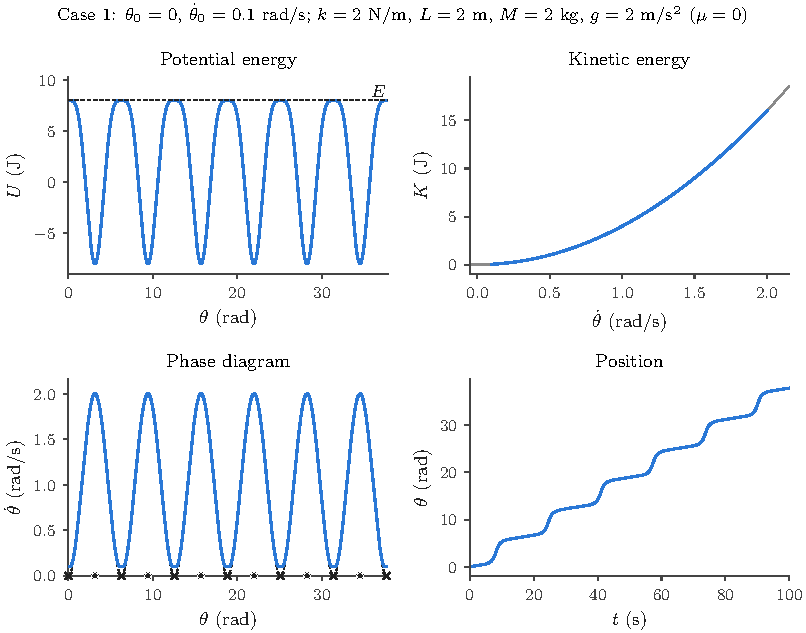
\includegraphics[width=0.78\textwidth]{figures/supplement/case1_en.pdf}
\caption{Case 1, critical coupling ($kL=Mg$, $\mu=0$): rotation just above the separatrix energy ($E/MgL=1.005$, $E_{\mathrm{sep}}/MgL=1.000$), with period $T=16.389$~s and critical slowing down near the degenerate upright position.}
\label{fig:case1}
\end{figure}

\begin{figure}[h!]
\centering
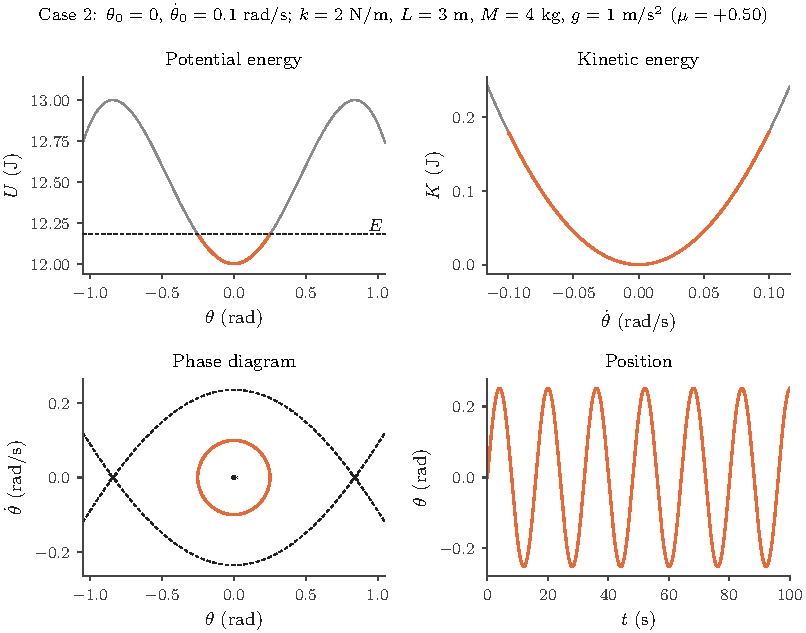
\includegraphics[width=0.78\textwidth]{figures/supplement/case2_en.pdf}
\caption{Case 2, stiff spring ($\mu=+0.50$): libration of amplitude $0.252$~rad inside the upright well ($E/MgL=1.015$, below $E_{\mathrm{sep}}/MgL=1.083$), with period $T=16.032$~s.}
\label{fig:case2}
\end{figure}

\begin{figure}[h!]
\centering
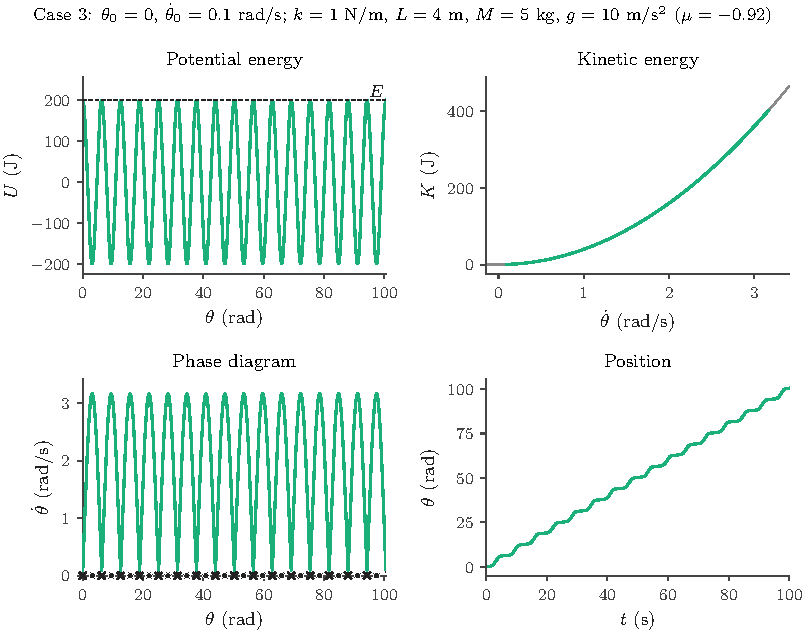
\includegraphics[width=0.78\textwidth]{figures/supplement/case3_en.pdf}
\caption{Case 3, weak spring ($\mu=-0.92$): rotation just above the separatrix energy ($E/MgL=1.002$, $E_{\mathrm{sep}}/MgL=1.000$), with period $T=6.272$~s.}
\label{fig:case3}
\end{figure}

\begin{figure}[h!]
\centering
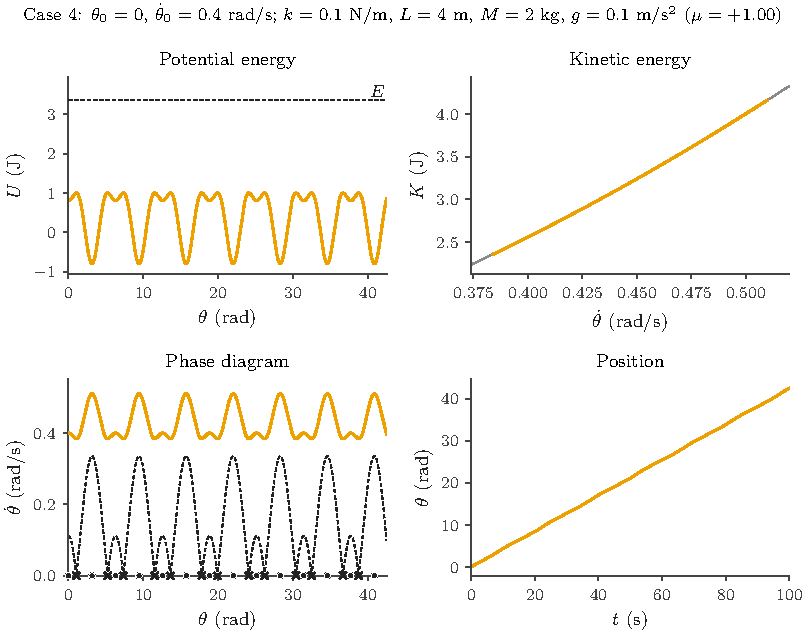
\includegraphics[width=0.78\textwidth]{figures/supplement/case4_en.pdf}
\caption{Case 4, stiff spring ($\mu=+1.00$): rotation far above the separatrix ($E/MgL=4.200$, $E_{\mathrm{sep}}/MgL=1.250$), with period $T=14.838$~s.}
\label{fig:case4}
\end{figure}

\begin{figure}[h!]
\centering
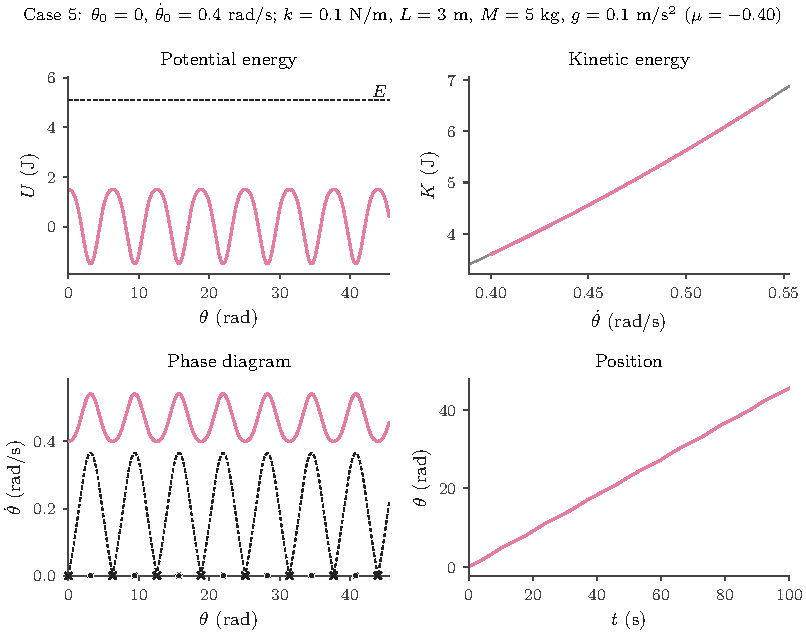
\includegraphics[width=0.78\textwidth]{figures/supplement/case5_en.pdf}
\caption{Case 5, weak spring ($\mu=-0.40$): rotation far above the separatrix ($E/MgL=3.400$, $E_{\mathrm{sep}}/MgL=1.000$), with period $T=13.742$~s.}
\label{fig:case5}
\end{figure}

\clearpage
%% ------------------------------------------------------------------------------------------
\section{Guide to the laboratory}\label{sec:guide}

The code archive, openly available at \url{https://github.com/faorjuelal/PIAR}, contains the Python package \texttt{piar}, the experiment and figure scripts, the unit tests, the interactive notebook, the browser-based simulation, the numerical results, and the source of the article. Table~\ref{tab:guide} relates every result to the script that produces it and to the files that store it. The scripts are run from the root of the archive, in the order of the table, after installing the dependencies listed in \texttt{requirements.txt} (Python 3.11 with NumPy 2.4.4, SciPy 1.17.1, Numba 0.67.0, PyTorch 2.14.0, \texttt{zuko} 1.6.0, scikit-learn 1.8.0, Matplotlib 3.10.9, and \texttt{cmcrameri} 1.10); the figure style requires a \LaTeX\ installation. All random seeds are fixed in the scripts. The experiments E1--E8 correspond to the scripts \texttt{e1\_cases.py} to \texttt{e8\_symmetry.py}. On two processor cores, E1 and E2 take about a minute each, the benchmark E3 about three hours in total, E4 about four minutes, E5 and E8 a few seconds each, E6 about sixteen minutes of Gaussian-process fitting, and E7 several minutes. The command \texttt{pytest -q} runs the ten unit tests described in Sec.~\mref{sec:lab}. The notebook \texttt{notebooks/PIAR\_Dashboard.ipynb} contains the interactive dashboard of Fig.~\mref{fig:dashboard}, and the file \texttt{web/piar\_simulation.html} runs the browser-based simulation without installation.

\begin{table}[!htbp]
\caption{Scripts of the laboratory (directory \texttt{experiments/}) and the results they produce.}
\label{tab:guide}
\centering\footnotesize
\begin{tabular}{>{\raggedright\arraybackslash}p{0.27\textwidth}>{\raggedright\arraybackslash}p{0.27\textwidth}>{\raggedright\arraybackslash}p{0.38\textwidth}}
\toprule
Result & Script & Output files\\
\midrule
Figs.~\mref{fig:model}--\mref{fig:portraits}, Table~\mref{tab:cases}, Figs.~\ref{fig:case1}--\ref{fig:case5} & \texttt{e1\_cases.py} & \texttt{results/e1\_cases.json}; \texttt{figures/fig\_model}, \texttt{fig\_cases}, \texttt{fig\_portraits}; \texttt{figures/cases/}\\
Secs.~\mref{sec:route}--\mref{sec:attractor}, Table~\mref{tab:chaos} & \texttt{e2\_chaos.py} & \texttt{results/e2\_chaos.json}, \texttt{e2\_chaos.npz}\\
Figs.~\mref{fig:route} and \mref{fig:attractor} & \texttt{fig\_chaos.py} & \texttt{figures/fig\_route}, \texttt{fig\_attractor}\\
Sec.~\mref{sec:attractor}, Table~\ref{tab:sym} & \texttt{e8\_symmetry.py} & \texttt{results/e8\_symmetry.json}\\
Fig.~\mref{fig:fprm_scheme} & \texttt{fig\_fprm\_scheme.py} & \texttt{results/fig\_fprm\_scheme.json}; \texttt{figures/fig\_fprm\_scheme}\\
Benchmark of Sec.~\mref{sec:results} & \texttt{e3\_fprm.py} (argument C0, C1, C2, or C3) & \texttt{results/e3\_C0.json}--\texttt{e3\_C3.json} and sample caches\\
Table~\mref{tab:fprm}, Fig.~\mref{fig:fprm} & \texttt{fig\_fprm.py} & \texttt{manuscript/tables/tab\_fprm.tex}; \texttt{figures/fig\_fprm}\\
Fig.~\mref{fig:reconstruction} & \texttt{e4\_reconstruction.py}, \texttt{fig\_reconstruction.py} & \texttt{results/e4\_reconstruction.json}, \texttt{e4\_reconstruction.npz}, \texttt{fig\_reconstruction.json}; \texttt{figures/fig\_reconstruction}\\
Secs.~\mref{sec:res_c1} and \mref{sec:res_physics}, Table~\ref{tab:lib} & \texttt{e5\_diagnostics.py} & \texttt{results/e5\_diagnostics.json}\\
Sec.~\mref{sec:res_c1}, Table~\ref{tab:fullgp} & \texttt{e6\_fullgp.py} & \texttt{results/e6\_fullgp.json}\\
Sec.~\mref{sec:res_engine}, Table~\ref{tab:cost} & \texttt{e7\_engine\_cost.py} & \texttt{results/e7\_engine\_cost.json}\\
Fig.~\mref{fig:dashboard} & \texttt{fig\_dashboard.py} & \texttt{figures/fig\_dashboard}\\
Tables~\ref{tab:C1}--\ref{tab:sym}, Fig.~\ref{fig:emb} & \texttt{make\_supplement.py} & \texttt{manuscript/supplement/}; \texttt{figures/figS\_embedding}; \texttt{results/benchmark\_runs.csv}\\
\bottomrule
\end{tabular}
\end{table}

\end{document}
